\chapter{Introduction}
\label{ch:intro}
\chaptermark{Introduction}

%\setcounter{equation}{0}
% ==========================================================================================================
With the advance of functional magnetic resonance imaging (fMRI) and other neuroimaging technique, the study of ongoing thought has gained wider interest in psychology and neuroscience in the past decade. The increasing research has given rise to heterogeneous views on how and why mind-wandering occurs, however, the detailed neural basis of the heterogeneity remains largely unclear. The current thesis explores the patterns of ongoing thought extending from well-studied off-task thought---mind-wandering---to task-related thought. The aim is to gain an understanding of the component processes of ongoing thought at task and rest. A flexible family resemblance view \cite{Seli2018} of ongoing thought will jointly identify patterns of the shared similarities, as well as unique features that drive the heterogeneity.

In this chapter, I walk through the conflicting behavioural literature of mind-wandering and discuss the theoretical accounts of ongoing thought. Next, I introduce the emerging neural evidence on the hierarchical organisation of cognition \cite{Margulies2016,Mesulam1998} and argue how overlapping component processes might facilitate ongoing thought. In closing, I introduce the overall methods used in the current research and how a multivariate approach helps to examine the family resemblance view of ongoing thought.

\section{Heterogeneity of ongoing thought}
\label{ch:intro:heterogeneity}
\sectionmark{Heterogeneity}

% lay out the component processing account and family resemblance view

Mind-wandering is particularly well-studied among all phenomena related to ongoing thoughts. Researchers aim to understand how the mind shifts between the external environment and internal thoughts unrelated to the here-and-now. 
The executive failure account is concerned with why some mind-wandering episodes occur to the detriment of the integrity of an ongoing task \cite{McVay2010}. In contrast to the executive failure view, the representational account seeks an understanding of how the mental content is generated \cite{Smallwood2016}. The two approaches have led to conflict in the mind-wandering literature. \citeA{Seli2018} has recently proposed a family resemblance view to incorporate different theoretical accounts under a common framework. In a family resemblance view, members of the ongoing thought family can have shared similarities along with unique features resulting in heterogeneity. The following section will introduce the evidence for construct overlap and shared processes of ongoing thought at task and rest.

\subsection{Heterogeneity in definitions}
Among types of ongoing thought, mind-wandering attracted the most interest as it concerns the ability to focus on the task at hand. Mind-wandering has been studied in a variety of related psychological domains, such as cognition, emotion, and neuroscience. Various lines of research have addressed the basic phenomenal characteristics of mind-wandering---
\begin{quote}
    \textit{a shift in the contents of thought away from an ongoing task and/or from events in the external environment to self-generated thoughts and feelings.}\\    
    \cite{SmallwoodSchooler2006,SmallwoodSchooler2015}.
\end{quote}
We are all familiar with moments when the train of thought shift away from the tasks at hand, and sometimes get annoyed by the mind-wandering episode. This intuition has lead to researches describing mind-wandering as an `attentional lapse' \cite{McVayJOEP2009, McVay2012}, implying the occurrence of mind-wandering is an unintended failure. When a study explicitly instructs the participant to perform a task, the time not focused on the task is considered as `mind-wandering'. Such research designs dismissed the possibility of voluntary engagement in the mind-wandering state. 

Recent investigations have found that mind-wandering can occur with or without intention \cite<see the review from>{SeliTiCS2016}. The participant can intentionally mind wander if they lack a motivation to engage in the experiment. When a simple yes/no question is asked about the mind-wandering state, the response cannot access the nature of the occurrence. When participants are asked about the nature of mind-wandering periods in a laboratory scenario, less than half of the mind-wandering is intentional \cite{SeliJoEP2015} due to the lack of motivation to complete the task \cite{SeliJoEP2015}, or the task is not mentally demanding enough to have all attentional resources allocated to the task \cite{SeliPsychScience2016}. The occurrence of intended and unintended mind-wandering can also be down to individual differences. Intentional and unintentional mind-wandering have been found to be differentially associated with attention-deficit/hyperactivity disorder \cite<ADHD;>{SeliADHD2015} and obsessive-compulsive disorder \cite<OCD;>{SeliOCD2017}. The work on the intention of mind-wandering demonstrates that there is indeed overlap in the various definitions and other components that contribute to the heterogeneity. 

\subsection{Heterogeneity in functional outcomes}

The family resemblance view suggests that complex thought can emerge from the combination of multiple overlapping processes. A myriad of mind-wandering research concerns functional outcomes. The current thesis proposes that the heterogeneous functional outcomes are evidence in support of a variety of component processes underlying ongoing thought. 

mind-wandering has been associated with poor executive control during working memory task \cite{McVayJOEP2009}. Individuals who mind-wandered more during fluid intelligent testing perform less well \cite{MrazekJoEP2012}. Mind-wandering leads to bad reading comprehension due to failure in the construction of the mental models of ongoing events \cite{Smallwood2008}. Comprehension ability is related to working memory capacity and mediated by the ability to suppress mind-wandering \cite{McVayReading2012, Unsworth2013}. Mind-wandering has been linked to unhappiness \cite{Killingsworth2010} and is an indicator of depression \cite{Smallwood2007}. The evidence above supports the highly disruptive nature of mind-wandering and its potential costs to cognitive performance.

In addition to exploring the costs of mind-wandering, researchers have discovered its potential benefits. Mind-wandering may facilitate a creative solution to an old problem \cite{Baird2012, Smeekens2016} and recovery from negative emotional states \cite{RubyPlos2013, PoerioFrontiers2016}. Mind-wandering relies on mental time travel---the metal capacity of remembering the past and imagining the future \cite{Stawarczyk2015}---and relies on neural mechanisms associated with the memory function \cite{DArgembeau2006,DArgembeau2015}. Mind-wandering can also refine personal goals \cite{Medea2016}, potentially through mental time travel. 

In summary, different functional associations arise from the same type of experience---mind-wandering. To reconcile this contradictory evidence, researchers have suggested that mind-wandering may encompass multiple states with differential contents and underlying cognitive architectures \cite{SmallwoodFrontiers2013}. Complex thought can emerge from the combination of multiple overlapping processes. 

\subsection{Heterogeneity in experiential profiles}

Self-report is commonly used to understand the content of mind-wandering thoughts and ongoing experience. The content of mind-wandering covers a wide variety of topics and modalities. The questions in the report address a number of dimensions of the ongoing experience, ranging from the state of attention, temporal content, social content and modality (i.e. thinking in words or images). Principle component analysis (PCA) formalised the statistically shared association between different aspects of the reports. 

Studies using PCA on such experience reports have revealed detailed experiential profiles. Temporal information is one common theme \cite{RubyFP2013,RubyPlos2013}. The content of mind-wandering is mainly future-focused \cite{Baird2011}, therefore mind-wandering often involves planning for the future goals of the individual. On the contrary, when the mind wanders in an unhappy mood, the content is drawn to events from its past \cite{Smallwood2011}. The form of spontaneous thoughts is likely to be imagery or verbal \cite{Gorgolewski2014,Smallwood2016}. 

In conclusion, the positive/negative-valence of the emotion of thought has a tendency to accompany with different temporal directions. These unique associations discovered through PCA suggested component processes at an experiential level. Investigation in experiential profiles is the first step to explore the commonality of various type of ongoing thought. 

% ==========================================================================================================

\section{Theoretical accounts of mind-wandering}
\sectionmark{Theoretical accounts}
\label{ch:intro:accounts}

The heterogeneity of mind-wandering has been formalised into two theoretical accounts. The executive failure account aims to understand the conditions that trigger or associate with ongoing thought \cite{Kane2012,McVay2010}. The representational account examines the mechanisms that give rise to different patterns of ongoing thought \cite{Smallwood2016}. In other words, the executive failure account examines why changes in ongoing thought happen, while the representational account seeks to explain how human generates ongoing thought while mind-wandering. The two accounts can be seen as competing theories of mind-wandering. However, in a family resemblance view, the two theoretical account potentially supports a singular phenomenon that is composed of multiple underlying component processes. 

\subsection{Executive failure account}
The executive failure account is concerned with a single aspect of mind-wandering, namely understanding why some mind-wandering episodes occur to the detriment of the integrity ongoing task. Mind-wandering occurs during attention-demanding tasks when control processes are insufficient to deal with the interference created by off-task thoughts \cite{Kane2012,McVay2010}. 
Under this view, mind-wandering results from a failure of attention to external tasks, rather than from the consumption of executive resources by internally generated thoughts. 
This research focuses on the negative effect of mind-wandering on the development of negative mood and task performance. Mind-wandering thoughts are mostly unhappy in ecologically valid scenario \cite{Killingsworth2010}. Depressive thinking correlates with the frequency of mind-wandering \cite{Smallwood2007}. 

In the executive failure view, mind-wandering reflects the momentary lapse in attention. The definition of attention lapse is a relatively slow response time to the task at hand, which is consistent with the mind-wandering indicator used in working memory capacity research \cite{McVay2012}. Mind-wandering has been considered the consequence of poor executive control during working memory task \cite{McVayJOEP2009}. Executive deficits and slow reaction times correlate with individual differences in working memory capacity and mind-wandering \cite{McVay2012}. The capacity to avoid mind-wandering during demanding tasks is a potentially important source of success on measures of fluid intelligence \cite{MrazekJoEP2012}. 

% neural basis
Task-based fMRI studies of attentional lapses have contributed to the functional neural processes to support the executive failure account. \citeA{Weissman2006} have described the neural mechanism associated with attentional lapses during a global/local selective-attention task. Brief attentional lapses are related to early activity in frontal control region including anterior cingulate cortex (ACC), right middle frontal gyrus (MFG), and right inferior frontal gyrus (IFG). Attentional lapses also suggest a failure to maintain perceptual representations. Reduced activity is found in the primary visual area. Activation of the default mode network \cite<DMN;>{Raichle2001,Shulman1997} has also been observed during a brief attention lapse. DMN is a set of brain regions composed of the medial prefrontal cortex(MPFC), posterior cingulate cortex (PCC) and angular gyrus (AG) as the core (REF), plus subsystems within medial and lateral temporal lobe \cite{Andrews-Hanna2010}. DMN is commonly referred as a task-negative network \cite{Fox2005}, associating with task-unrelated thought and mind-wandering \cite{MasonScience2007,Christoff2009}. The lapses increase demands on the frontal-parietal control network to redirect attention. Ventral frontal-parietal regions, including right temporal-parietal junction (TPJ) and right IFG, respond during recovery from lapses \cite{Corbetta2002,Weissman2006}. 

\subsection{Representational account}

The representational account concerns the generation of content during mind-wandering, suggesting that mind-wandering is not merely a mindless state. The ability to generate information without task-constrains is consistent with the productive functional outcomes of mind-wandering, such as creativity \cite{Baird2012,Smeekens2016} and social-temporal problem-solving \cite{RubyPlos2013,PoerioFrontiers2016,Medea2016}. 

The internal representation of semantics and episodic memory is associated with brain regions highly overlapping with DMN. The brain regions involved in semantic processing include left AG, lateral and ventral temporal cortex, left dorsal MPFC, left IFG, left ventral MPFC, and PCC \cite{Binder2009,Lambon-Ralph2017}. Dorsal and ventral MPFC show high activity at rest and are associated with personally relevant information \cite{Gusnard2001}. Studies of spontaneous thought suggest that PCC is an integrational hub of information from medial and lateral temporal lobes \cite{Smallwood2016}. Integration of the hippocampus with the DMN facilitates mental time travel \cite{Karapanagiotidis2017}. This representational process is not unique to mind-wandering. \citeA{VatanseverPNAS2017} demonstrated that the application of a newly acquired rule is associated with memory representation related brain regions such as hippocampus and PCC. 

DMN demonstrates both integrative and segregating pattern with the sensory systems to support the representational process, such as semantic processing \cite{Binder2009,Krieger-Redwood2016}, episodic recollection \cite{Rugg2013}, mental time travel \cite{Schacter2007}. A common requirement of these cognitive processes is the focus on previously-encoded knowledge, as opposed to information in the external environment.
The integrative and segregating modes of DMN are closely allied to perception-decoupling and conceptually-guided cognition \cite{Murphy2018}. 
% decouple
The ability of DMN to functionally decouple from perceptual dominant systems allows DMN to operate in an offline manner dissociated from the external input \cite{Smallwood2013}. This is consistent with recent observations of the functional organisation of the cortical surface \cite{Margulies2016} where the DMN is far from primary visual and motor cortex in terms of Euclidean distance and functional connectivity. 
% integration
In addition, the integrative pattern between DMN and sensorimotor regions might be supported by increased abstraction and integration along the ventral visual system, ending in a conceptual hub in the ATL \cite{Lambon-Ralph2017}. 
This view is also consistent with the observation that a gradient from unimodal to transmodal cortex \cite{Margulies2016} corresponds to increasingly abstract and complex cognitive tasks, where the influence of specific features linked to stimuli in the immediate environment is reduced \cite{Mesulam1998,Buckner2013,Margulies2016}.

% ==========================================================================================================
\section{Neural hierarchies}
\sectionmark{Neural hierarchies}
\label{ch:intro:neural}

The executive failure and representational accounts stemmed from distinctively different psychological research approaches to understand mind-wandering. The attentional system and the DMN are the common neural processes of both theoretical accounts, but interacting in a seemly contradicting manner. In the executive failure account, the attention-related system deactivates with poor task performance, accompanied by the activation in the DMN; while in the representational account, the attention system and the DMN work together to maintain the internal representation of memory. 
One possible reason for this conflict could be that under different global neural configurations, DMN might support different cognitive functions. 
In the current section, I discuss the progress of functional neuroimaging study towards a hierarchical view of neural systems corresponding to the family resemblance account.

\subsection{Historical perspective}

Research on brain organisation has been dominated by two opposing views---\textit{functional specialisation} and \textit{functional integration}. Functional specialisation emphasises that small, distinguishable brain regions are solving distinct problems \cite{Kanwisher2010}. Studies of cognitive impairments in people with focal brain lesions provides extensive evidence for the localisation of some functions in the human brain, such as the role of mid-fusiform gyrus in processing faces \cite{Iaria2008} and left Brodmann areas 44 and 45 (left IFG) in speech production \cite{Broca1861}. Single-cell recordings and microscopic tissue examination revealed the segregation of occipital visual cortex \cite{Zeki1978}. Overall, the approach used to yield localise brain function shares one important similarity. The methodology leads to interpretations based on non-overlapping, discrete region as the basic compartments of brain organisation. 

The recent focus in neuroscience has shifted from restricted regions to network organisation. Functional integration emphasises that cognitive function is enabled by a complex interplay between these distinct brain regions \cite{Sporns2014}. Biological neural network properties are an important source of electrophysiological oscillations. Independent component analysis (ICA) became the workhorses of network discovery in neuroimaging\cite{Beckmann2005}. Functional connectivity \cite{FristonHBM1994} and graph theory \cite{Rubinov2010} application to functional neuroimaging provided non-biophysical model of brain organisation. Recent advances in the field of human connectomics have revealed multiple large-scale networks, each characterised by distinct functional profiles \cite<e.g.>{Yeo2011}. In contrast to the specialisation of regions, cross-regional integration is the central approach to understanding the basic architecture of brain organisation.

Discovery from functional specialisation and integration has both revealed spatial gradients in brain organisation. Advances in mapping local stream such as vision \cite{Zeki1978} have revealed spatial gradients extending along adjacent cortical regions. Stepwise functional connectivity analysis demonstrated transitions from primary sensory cortices to higher-order brain systems for perceptual integration in the human brain \cite{Sepulcre2012}. The diffusion embedding analysis on connectivity data in humans and the macaque monkey reveals the principal gradients of whole brain topographical organisation \cite{Margulies2016}. The discovery of multiple whole-brain functional configurations provides speculations on hierarchical relations among inter-plays of large-scale networks.

\subsection{Abstract rules governing}
\citeA{Duncan2010} discovered a common pattern of activity in the prefrontal and parietal activity of the human brain in response to a diverse cognitive challenge. He revealed that the governance of cognitive control is the multiple-demand network (MDN) covering regions in the attention system and the frontoparietal network (FPN). This involves cortices in and around the posterior part of the inferior frontal sulcus (IFS), in the anterior insula (AI) and adjacent frontal operculum (FO), in the pre-supplementary motor area (pre-SMA) and adjacent dorsal ACC, and in and around the intraparietal sulcus (IPS). Similar multiple-demand patterns are identified in resting state data described as `task-positive' \cite{Fox2005}, as opposed to the `task negative' pattern---the DMN. The MDN activity is consistent with the neural model \cite{Weissman2006} proposed to explain the executive failure account of mind-wandering \cite{McVay2012}. The antagonistic roles of DMN and MDN seem to be essential to \textit{abstract rules governing}.  

The past research paradigms segregated complex cognition into isolated operations such as working memory capacity \cite{Vogel2004} and response inhibition \cite{Aron2004}. Complex, multi-component behaviour should be examined to understand the central role of control in realistic behaviours. Tasks with multiple-demand properties, such as intelligence tasks, examine abstract thinking, multi-modal or feature integration skills, a working memory. The current thesis speculates that multiple-demand neural patterns manifest family resemblance property for the executive control. 

\subsection{Sensory integration/segregation}
\citeA{Mesulam1998} observed that the primary visual and auditory cortices form a spatially continuous organisation towards the hetermodal cortices of the frontal and parietal lobes. He hypothesised that the hetermodal regions are selectively converging the input from unimodal regions to form abstract information, forming a hierarchical polarity. This viewpoint was examined by \citeA{Margulies2016} through a meta-analysis of cognitive function of the first principle gradient of the human brain. The first gradient anchors the unimodal regions at one end and the transmodal regions in FPN and DMN at the other. The continuum characterises a spectrum from unimodal to transmodal activity in a meta-analysis on cognitive function tasks, with sensory-driven tasks on the unimodal end and the abstract reasoning task on the transmodal end.

In this \textit{sensory integration/segregation} view, the FPN and DMN are functionally adjacent. Empirical research in cognitive neuroscience has found a similar hierarchy in mental scene construction \cite{Villena-Gonzalez2018} and higher-order conceptual representations \cite{Murphy2018}, which are essential functions supporting the representational account of mind-wandering. Recent research on the role of DMN has provided support for a global integrative view in which DMN forms the highest level in a neural hierarchy \cite{Margulies2016}. Investigation of the activity of DMN indicates major revisions of cognitive context when conducting an explicit task. \citeA{VatanseverPNAS2017} recently demonstrated that the integrative role of DMN with primary visual cortices and hippocampus facilitate a rapid and adaptive rule learning. 
Patterns of cognition with neural activity located along the gradient between the sensorimotor system and DMN will tend to share key characteristics, giving rise to a family resemblance in memory-guided and perception-guided representations.

\subsection{Integration of hierarchical configurations}

The neural hierarchy of \textit{abstract rule governing} and \textit{sensory integration/segregation} have described contradictory views of the organisation of DMN and FPN. In the \textit{sensory integration/segregation} view, reflecting sensory integration/segregation, these two networks are near-neighbours. Yet in the \textit{abstract rule governing} view, they tend to be in opposition.
The commonality of the two views lies in the attention regulation role of FPN. DMN represents the lack of control in the abstract rule governing, while it serves as the integrational hub of information from FPN in the sensory integration view. Interestingly, these two neural hierarchies are consistent with the contradictions between the \textit{executive failure} and \textit{representational} account in ongoing thought, where mind-wandering results from poor task performance in executive failure account, but the representational account can explain the benefits and generation of mental representations in ongoing thought. 
The two neural hierarchies may describe the complementary whole-brain activity of these two theoretical accounts of ongoing thoughts. 
% Again, making this completely explicit could help. Mind-wandering at the expense of an ongoing task is characterized by the opposition between DMN (task-negative) and FPN (task-positive networks). However, the more nuanced view that DMN supports some demanding cognitive states such as imagination and creativity, might be related to the positive benefits of mind-wandering and might be captured by the similarity between DMN and FPN in terms of their heteromodal nature.

The study of ongoing thought is in need of an integrative approach to pool related cognitive functions and whole brain patterns under a cohesive narrative. The hidden family resemblance may resolve the conflict in theoretical views of ongoing thought. Recent studies of the MDN supports the family resemblance view that a component can possess multiple states. %
\citeA{Crittenden2015,Crittenden2016} demonstrated the involvement of both MDN and DMN in a rule switching task. Using multi-voxel pattern analysis, two tightly knitted subprocessing with distinct role have been revealed in multiple-demand tasks \cite{Crittenden2015}, while the coupling of the two networks has shown a board representation of abstract rules \cite{Crittenden2016}. 
The context dependency of the function of DMN implies the importance of the whole brain pattern to understand complex behaviour. Further development of the neuro-cognitive model is crucial to achieving a more granular view of ongoing thought \cite{Mittner2016,SmallwoodFrontiers2013}. 

% ==========================================================================================================
\section{The current thesis}
\sectionmark{The current thesis}

The conflicts in the mind-wandering literature arise from the heterogeneous, unconstrained nature of ongoing thought. To date, research on ongoing thought consists of investigations on three important aspects: experience, neural profile, and cognition (\cref{fig:intro:fig1}). A detailed description of spontaneous thought is needed to confirm the experience of ongoing thought. The neural organisation serves as the intrinsic biological basis of cognition. Finally, established cognitive measures link functional outcomes to the experiential profiles. 

\begin{figure}[H]
    \vspace{10pt}
    \centering
    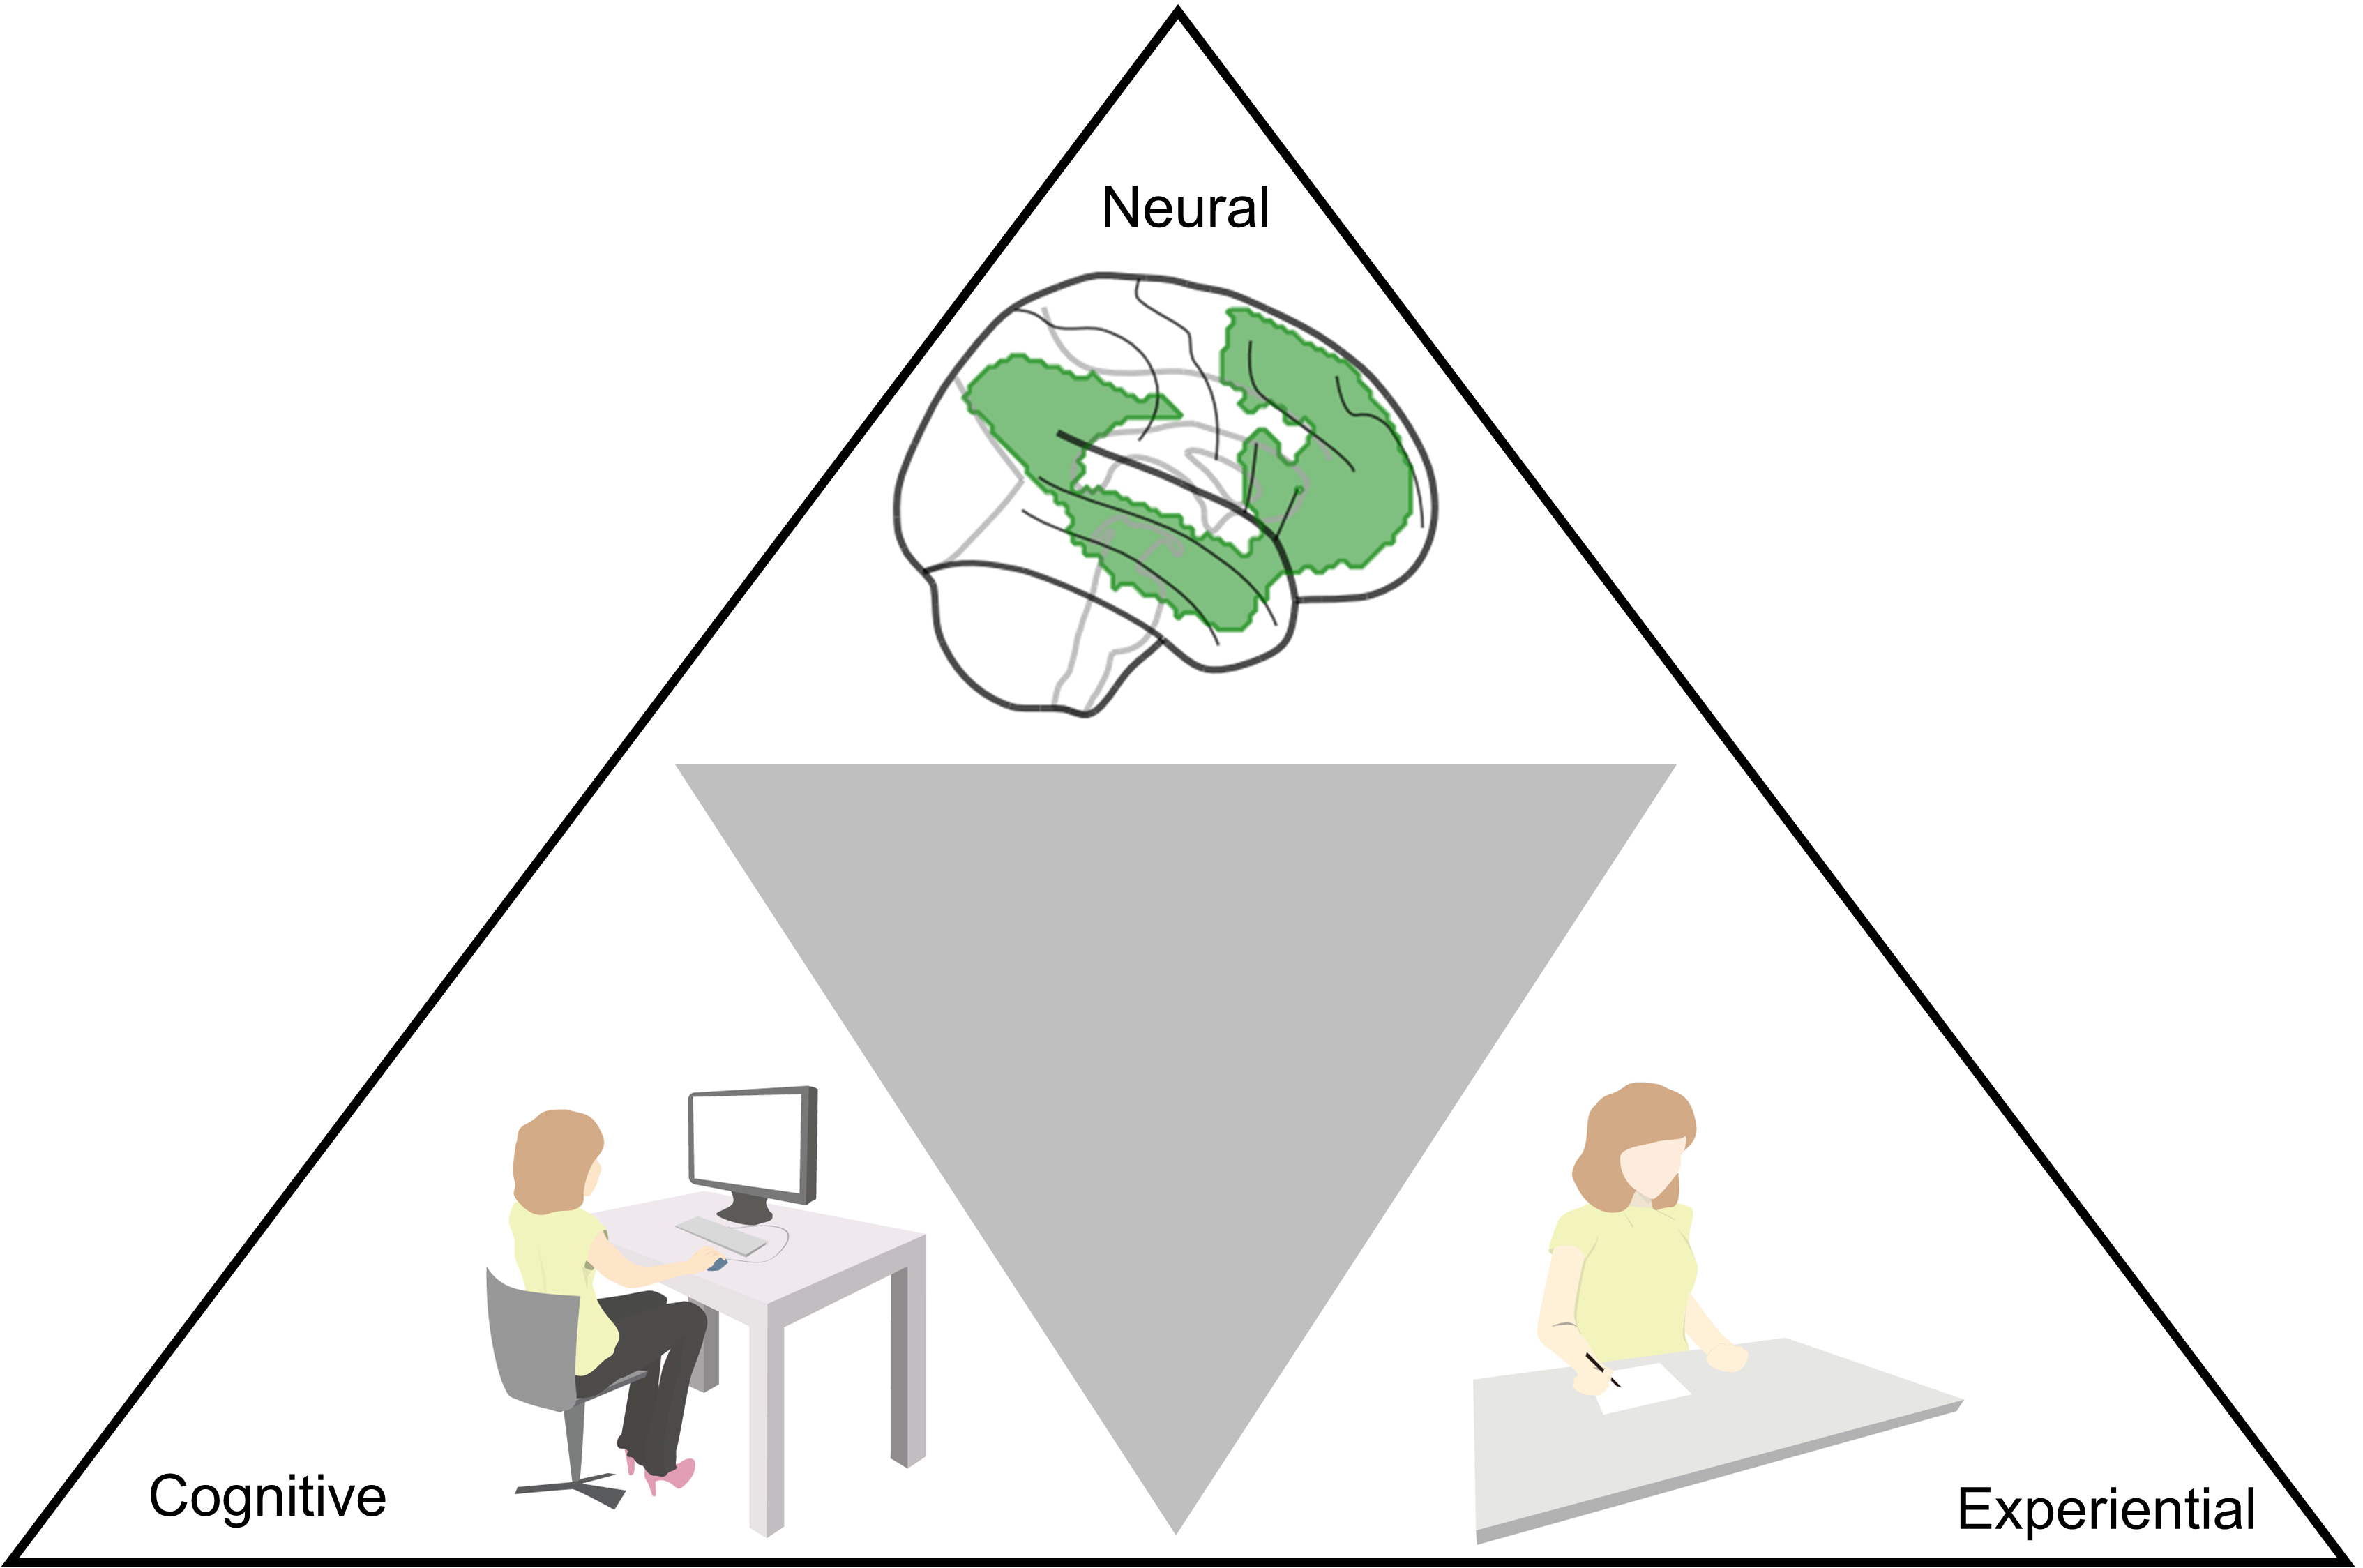
\includegraphics[width=0.8\textwidth]{intro/image/thesisfig1.png}
    \caption{Schematic of the thesis}
    %\vspace{-10pt}
    \label{fig:intro:fig1}
\end{figure}

Studies targeting relationships within a single aspect of ongoing thought (i.e. experiential, neural or cognitive) might only capture few potential members of the family of ongoing thought. When the family members sampled possess non-prototypical features, the discovery could be presented as rival theories. For instance, the study of ongoing thought associated with creativity and working memory are presented as conflicts of mind-wandering profiles. With an understanding of the component processes composing the family property, the heterogeneity of ongoing thought may be interpreted as exemplars of component processes rather than conflicts. 

The current thesis adapts a multivariate approach as the first step towards a family resemblance view of ongoing thought. A multivariate approach can include observations on a wider variety of behavioural profiles, thus preventing over-representing an exemplary as the whole category. Multidimensional experience sampling \cite<MDES;>{Medea2016, RubyPlos2013, Smallwood2016} is the main technique of experience profile assessment to capture the various aspects of thought. Resting-state functional connectivity is used to describe the trait-like neural feature of each individual. The tasks selected measure cognitive functions documented in the past mind-wandering literature, including executive control, fluid intelligence, episodic memory, semantic memory, and information generation. Finally, canonical correlation analysis \cite<CCA;>{Hotelling1936} is the conjoined-decomposition method of choice to explore the multivariate patterns of mind-wandering. Here I present the overview of the ongoing thought measure and the benefit of CCA used in the thesis.  

\subsection{Method of acquiring experience}

In the current thesis, both online and retrospective method is used to acquire the content of ongoing thought in laboratory scenario. In the online measure, MDES uses thought probes to record participants' experiences during a given task. Thought probes appear during the task in a semi-random fashion. The online measure captures spontaneous thought in, possibly, both off-task and task-focused moments. In the first and third empirical studies, the averaged momentary report from MDES is used to capture the trait-like features of spontaneous cognition. In the second empirical study, New York Cognition Questionnaire \cite{Gorgolewski2014} is used to acquire the trait-like multidimensional mind-wandering thought content during a 9-minute resting state fMRI session. The retrospective method measures the summary of the mind-wandering experience during a specified time period. The benefit of retrospective measure is that no interruption during the given task or the ongoing thoughts will happen. The trait-level features of mind-wandering are accessed in the retrospective report. 

A hybrid of go/no-go task and n-back task was used to manipulate working memory capacity while recording online experiences \cite{Konishi2015, Medea2016}. The earlier version has used numbers as the test items \cite{SmallwoodNI2013,SmallwoodPlos2011}. The majority of the experiment consists of nontarget presented in neutral colour and a small proportion of targets. Participants are instructed to judge whether the target number is odd or even. In the \textit{choice reaction time} (i.e. 0-back) condition, the judgement is made when the number changes colour; in the \textit{working memory} (i.e. 1-back) condition, participants judge the number on the previous screen when presented with a question mark. The improved version is proposed by Konishi and colleagues \citeyear{Konishi2015}, replacing numbers with two 2-dimensional geometric shapes separated by a vertical line. Each pair consists of two shapes among a circle, a triangle, and a square, each in two different left/right configurations. In the 0-back condition, the target is flanked by one of two shapes, and participants indicate which shape matches the target shape. In the 1-back condition, the target is flanked by two question marks, and participants match the target shape to the prior trial. 

\subsection{Content of experience}

For the purpose of capturing the momentary evolution of thoughts during experiments, experience sampling \cite{Kahneman2004} is a commonly used technique. Experience sampling is conducted during an external task, such as reading \cite{Franklin2011}, go/no-go task \cite{Christoff2009}, and n-back task\cite{Kane2007}. The list of questions needs to be short and concise to minimize interruption of the external task. To access the complex, heterogeneous content of spontaneous thoughts, the current thesis employs MDES \cite{Medea2016, RubyPlos2013, Smallwood2016}. MDES expanded the thought probe from an on/off task question to a collection of dimensions related to a wide range of questions about the form and content of thoughts. The idea of MDES is based on various questionnaires to understand the content of mind-wandering thoughts retrospectively, such as the Dundee Stress State Questionnaire \cite{Matthews1999}, Amsterdam Resting-State Questionnaire \cite{Diaz2013}, the resting state questionnaire \cite{Delamillieure2010}, and the New York Cognition Questionnaire \cite{Gorgolewski2014}. The questionnaires above include more than 20 items, providing comprehensive coverage of thought content. Direct implementation of the retrospective questionnaires listed above is not practical for experience sampling. 

The current version of MDES is based on the 10-question set used in \citeA{Medea2016} and \citeA{Smallwood2016}. In the previous work, the questions are separated into content and form aspects of the ongoing experience. PCA was used to extract latent linear structure in the spontaneous thought report. Each participant has a set of identified principle components concluding the average momentary state of all the sampled time period. The current version includes both form and content questions in one set with three extra questions. The average score of each thought dimension indicates the average momentary state of ongoing thought. Unique associations among the questions are expected to capture the family resemblance at an experiential level. 

% 

\subsection{Conjoined decomposition of brain and cognition}

Despite being invented in the 30s, CCA has not aroused researchers' interests due to the lack of practicality. With the advance in computing resource and enriched data size, CCA has gained popularity in neuroimaging research. Three characteristics of CCA make it the method of choice. Firstly, CCA can be understood as a natural extension of PCA to two variable sets, but mutually linked by a joint correlation criterion (see \ref{ch:methods:intuitions:1} Joint information compression). Such extension enables the exploration of neuro-experiential component processes of the ongoing thought family. Secondly, CCA does not distinguish between the two variable sets during the information compression process (see \ref{ch:methods:intuitions:2} Symmetry). The identified dual-component dimensions correlate two aspects of the data together without indication of causality between neural function and cognition. Finally, CCA is capable of estimating more than one corresponding component pair from the two variable sets (see \ref{ch:methods:intuitions:3} Multiplicity). More than one pair of meaningful decomposition can be found, giving it the potential to examine the heterogeneity of mind-wandering content and their functional outcome. 

While CCA provided useful features to explore ongoing thought, its sparsity variation overcomes two technical issues of CCA application. Performing feature selection with sparsity improve the interpretability of the data and model fit. The data with more number of features than samples is accompanied with consequences of the so-called curse of dimensionality---the more dimensions are added to a data set, the less explanatory value a sample would have \cite{Domingos2012}. The number of functional connectivity measure can easily exceed the number of samples. In sum, SCCA allows decomposition on functional connectivity measures without sacrificing data richness or introducing difficulties in interpretation following data compression. The advantage and disadvantage of CCA and its variation are discussed in the next chapter.

The current thesis adopts the sparse variation of CCA \cite<SCCA;>{WittenSCCA2009} to resolve arguments related to the component processes under the family resemblance view. Most studies of ongoing thought have only focused on its relationship with one cognitive outcome at a time. As a consequence, mind-wandering is treated as a singular construct of all off-task ongoing thought. Studies on contents of ongoing experience have shown the diversity of information using self-report methods. Based on the heterogeneity of content, ongoing thought can be a collection of various type of spontaneous thoughts. Adopting a multivariate method has the potential to identify family resemblance among the heterogeneity of ongoing thought, and to begin the research on the ontology of the component processes of ongoing thought. % mention the relevance of the method

% ==========================================================================================================
\section{Summary and thesis outline}
\sectionmark{Summary}
Human cognition has the capacity to generate thoughts loosely related to the external world. However, researchers have not understood the mechanism behind the consequences of ongoing thought. The heterogeneity of functional outcomes has been a controversial and much disputed subject within the field of mind wandering research. Extensive research has shown that both costs and benefits to cognitive functions are associated with mind wandering. Negative consequences include reduced attention, poor task performance, unhappiness, and depression. The related positive outcomes include creative problem solving, planning personal goals, and recovery from negative emotion.

Most studies of mind wandering have only focused on one cognitive outcome at a time. Mind-wandering is treated as a singular construct. Studies of the contents of spontaneous ongoing thoughts have shown the diversity of information using self-report methods. The temporal content of ongoing thoughts can be future- or past-focused. The topic can be on personal issues or task related. Based on the heterogeneity of content, ongoing thoughts can be a family of various type of spontaneous thoughts with essential shared features. The lack of understanding of family resemblance results in conflicts in ongoing thought literature.

In the past decade, the neural basis of unconstrained processes has become the centre of the topic. DMN is the commonly engaged large-scale network. The extensive literature has documented the task-negative trait of DMN. The executive failure account of mind-wandering is in line with the task-negative view of DMN. However, the role of DMN in the memory representation account of ongoing thought is unresolved. Recent literature on neural hierarchy has cast a different light on the function of DMN. The highest-level abstract and heteromodal cognitive functions are associated with DMN, whereas perception and motor-related regions are related to sensory processing. This new view provides a clue to investigate the representational account of ongoing thought.

The conflict in the mind-wandering literature is related to the one-to-one matching between ongoing thought and the brain or behaviour. To paint the full picture of ongoing thought, a multivariate method will help incorporate the three aspects mentioned above: cognition, experience, and neural basis. The current thesis adopts SCCA to resolve arguments related to heterogeneity in mind wandering. With advances in computing resources and enriched data size, CCA has gained popularity in neural imaging research. The motivation of the current thesis is to resolve the conflict in the ongoing thought literature. Based on the recent research on neural hierarchies of cognition, the current thesis argues that regions beyond DMN contribute to the cognitive process underlying ongoing thought. The analysis, therefore, incorporates the functional organisation of large-scale neural networks as the main neural measure. The aim is to present evidence supporting of the family resemblance view and to begin research on the ontology of the component processes in ongoing thought. An outline of the remaining chapters is listed below:

\subsection*{\cref{ch:methods}: Canonical correlation analysis}

Canonical correlation analysis is introduced as the main method of the thesis. This review focuses on the potential applications in neuroimaging research. The features and applications of this multivariate method are outlined, followed by a discussion of the methods' interpretations and limitations. 

\textit{This chapter is under preparation for publication. } 

\subsection*{\cref{ch:study1}: Exploring the heterogeneity of ongoing thought}
Heterogeneity of mind-wandering leads to conflicting views about its functional outcomes in behavioural studies. Default mode network is commonly associated with the emergence of mind-wandering. SCCA conjointly decomposed functional connectivity patterns of DMN and thought reports, revealing unique neuro-experiential components. The study then revealed that the neuro-experiential components each associated with unique cognitive task measures. The various connectivity configurations within DMN are associated with different types of ongoing thought and specific functional outcomes.

\textit{This chapter is published in Psychological Science.}

\subsection*{\cref{ch:study2}: Population variation in the associations between large-scale networks and experiences}
Unconstrained cognitive processes have two faces. The representational account argues that the primary sensory brain regions decouple from DMN to facilitate memory representation; whereas the executive failure account shows lapses in attention are related to the demands on attention system and activation of DMN. We used SCCA to extract related whole-brain functional connectivity patterns, profiling the neuro-experiential components of unconstrained cognitive processes. Examining the association between demanding cognitive tasks and neuro-experiential components, the study revealed evidence supporting both the representational and executive failure accounts.

\textit{This chapter is published in NeuroImage.}

\subsection*{\cref{ch:study3}: Inhibition of prior information contributes to internal content representation}
Various cognitive functions are involved in the generation of internal experiences. The study of the functional outcomes is often conducted in a manner of one-to-one mapping. The heterogeneous cognitive outcomes are discussed as conflicts rather than the complex details driving the diversity of ongoing thought. In \cref{ch:study3}, we explore the intrinsic whole-brain neural basis of the cognitive functions supporting the unconstrained generation of spontaneous thoughts.  With SCCA we describe the conjoined decomposition of cognitive function and resting state functional connectivity. Similar to \cref{ch:study2}, this study explored the unconstrained neuro-cognitive mechanism underlying the various dimensions of ongoing thought.

\subsection*{\cref{ch:discussion}: General discussion}
The overarching themes of the thesis are discussed and linked to specific results throughout the thesis. Future research directions are inspired by the findings and limitations of the current thesis based upon the key questions which this thesis attempted to answer:

\begin{itemize}
    \item Why does ongoing thought show both costs and benefits? 
    \item Can functional neural hierarchy explain the heterogeneity?
    \item Is the family resemblance view viable for ongoing thought?
\end{itemize}


% ==========================================================================================================
